Calcule el volumen de un cono de radio $r$ y altura $h$.

\nopagebreak
\begin{align*}
\text{Generado por la rotación de la recta } y = \frac{r}{h}x \text{ alrededor del eje } x \text{ en } [0,h]. \\
V &= \pi \int_{0}^{h} \left(\frac{r}{h}x\right)^2 \, dx \\
&= \pi \frac{r^2}{h^2} \int_{0}^{h} x^2 \, dx \\
&= \pi \frac{r^2}{h^2} \left[ \frac{x^3}{3} \right]_{0}^{h} \\
&= \pi \frac{r^2}{h^2} \frac{h^3}{3} = \frac{1}{3} \pi r^2 h
\end{align*}

\[
\boxed{\displaystyle \frac{1}{3} \pi r^2 h}
\]

\begin{center}
    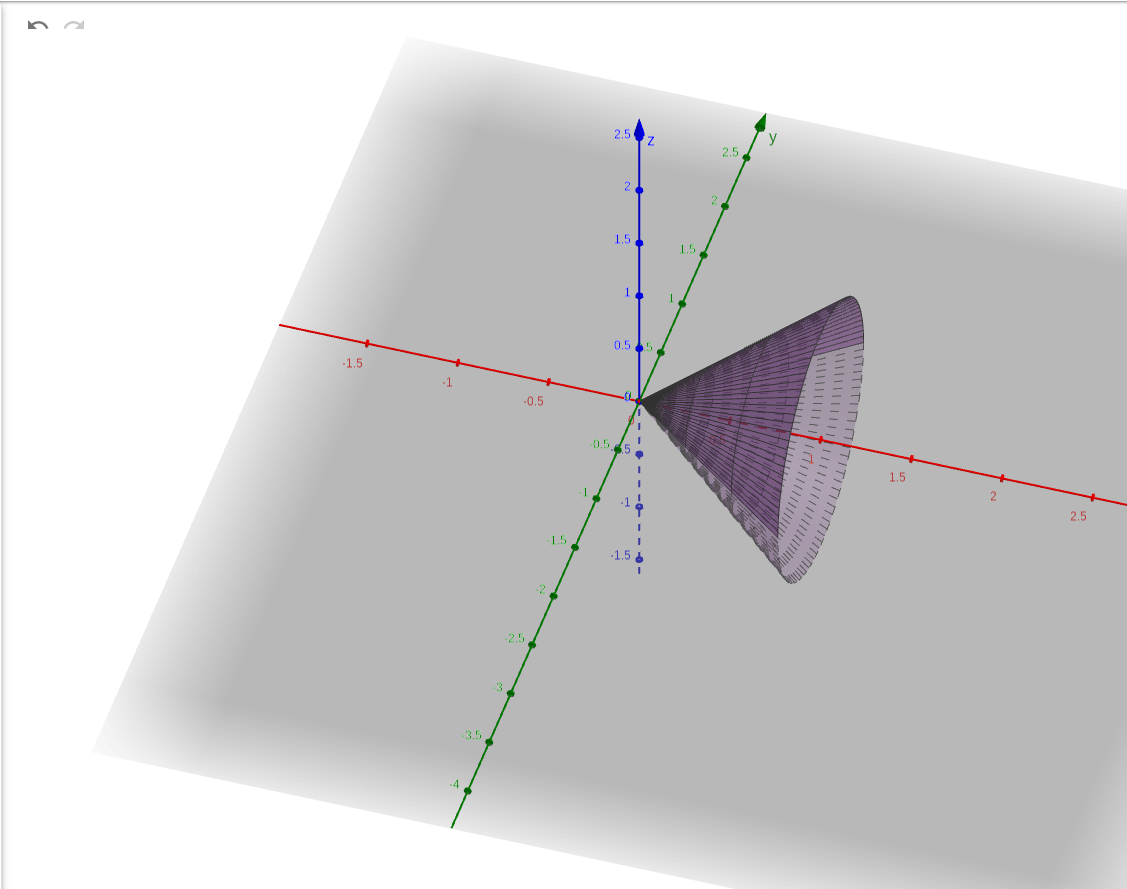
\includegraphics[width=0.5\textwidth]{Graficas/ejer31.png}
\end{center}
